\documentclass[twocolumn]{aastex62}

\newcommand{\vdag}{(v)^\dagger}
\newcommand\aastex{AAS\TeX}
\newcommand\latex{La\TeX}
\usepackage{amsmath}
\usepackage{physics}
\usepackage{hyperref}
\usepackage{natbib}
\usepackage[T1]{fontenc}
\usepackage[english]{babel}
\usepackage[utf8]{inputenc}
\usepackage{wasysym}

\begin{document}

\title{\Large Numerical Orbital Mechanics Simulations of the Solar System}

\author{Håkon Tansem}

\author{Nils-Ole Stutzer}

\author{Bernhard Nornes Lotsberg}

\begin{abstract}
We implement an $N$-body simulator to solve the motion of objects in the 
solar system. We compare the performance of the forward Euler and 
velocity Verlet numerical schemes. In this case the Velocity Verlet 
outperforms the forward Euler scheme as it has an error of $\sim 3$ 
orders of magnitude lower due to its symplectic nature conserving 
constants of motion in a Hamiltonian system.
In this simulation the Earth's escape velocity from the Sun is found as 
in the interval $v\in (8.86, 9.50)$ AU/Yr, which corresponds well with 
the analytically derived value of $v\approx 8.88$ AU/Yr. We also implemented a general relativistic correction term in Newton's gravitational force to calculate the precession of Mercury's orbit. Our results of approximately $450400$ arcseconds per century deviates a large amount from the observed precession motion of approximately $43$ arcseconds when subtracting precession due to other effects like planetary interactions. Further investigations of systematic errors is needed for our method to resolve small scale motions like the perihelion precession of Mercury's orbit.
\\\\
Github repository containing source code for this paper can be found here:\\ \url{https://github.com/hakontan/FYS4150-Project-5}

\end{abstract}

\section{Introduction} \label{sec:intro}
Celestial mechanics is a physical problem that has intreeged mankind since the
day of time. It has fascinated astronomers since night time observations done by
the antient greeks, through Galileo Galilei's studies of Jupiters moons in the
Renaissance, to todays detailed observations and simulations. At the present
date one can do detailed numerical simulations of the motion of planets and
other celestial objects, so as to predict their motion many centuries into the
future.

In this paper we will study how the celestial bodies in our Solar System
interact using two different numerical methods for solving the coupled
differential equations of motion discribing their movement. We will look at the
classical Forward Euler and the more advanced Velocity Verlet methods, and
compare them. In addition we will study different versions of the gravitational
force to see how it affects the planets orbit, and also we will see what happens
to the Earth's and Sun's motion if Jupiters mass is changes. Last we will study
Mercury's perihelion precession.

We will present theory and its implementation in the Method section. The results
of our study will be presented and discussed in the Results and Discussion
section respectively.


\section{Method} \label{sec:method}
\subsection{The Gravitational force and the Equations of Motion}\label{subsec:gravity}
The motion of celectial bodies in the solar system are governed by one single
force, being the gravitational force. In Newtonian physics this is written as
\begin{align}
    \vec{F} = -G\frac{Mm}{r^3}\vec{r},
\end{align}
where $F$ is the force between two masses $M$ and $m$ separated by a distance
$\vec{r}$ ($r = |\vec{r}|$) and $G$ is the gravitational constant. More
generally when having more than just two celectial bodies ($N$ bodies), the force on one of
them $m_i$ is simply the sum of the gravitational force from all the other
bodies $m_j$. Thus we have the total gravitational force 
\begin{align}
    \vec{F}_i = \sum_i^N \sum_{j\neq i}^N -G\frac{m_im_j}{|\vec{r}_j - \vec{r}_i|^3}(\vec{r}_j - \vec{r}_i) = m_i \vec{a}_i = m_i \ddot{\vec{r}}_i,
    \label{eq:newtonian_gravity}
\end{align}
where we used Newton's second law to find the acceleration. In this $N$-body problem
celestial bodies are interacting with each other, affecting each others motions.
When simulating our Solar System, it is often common to let the Sun be static at
the origin due to its mass being many orders of magnitude larger than that of
the planet, limiting its motion to a small wiggle. We will however include the
Suns motion in our simulations, as it reflects reality better than having it
static. 

When simulating the motions of the celectial bodies according to the force
(\ref{eq:newtonian_gravity}) it is convenient to chose a scaling more suited to
the scales of the Solar System. To find such a scaling we consider the
gravitational force between Earth and the Sun in a circular orbit. We then get 
\begin{align}
    F = G\frac{M_\oplus M_\odot}{r^2} = \frac{v^2}{r}M_\oplus,
\end{align}
using that gravity equals the centripetal force in a circular orbit. Since we
know that for a circualr orbit $v = \frac{2\pi r}{T}$, for an orbital periode $T
= 1\rm{yr}$, we get that the gravitational constant becomes
\begin{align}
    G = 4\pi^2 \frac{\rm{AU}^3}{\rm{yr}^2 M_\odot},
\end{align}
since the relative Sun-Earth distance in a circular orbit is $1\rm{AU}$. Thus we
use units solar masses $M_\odot$, astronomical units $\rm{AU}$ for distances and
years
$\rm{yr}$ for time, as they are far easier to handle. 

In order to solve the equations of motion we can write the second order ordinary
differentail equation (ODE) as a system of two coupled first order equations.
Further more as the equations are vector equations, we can write the coupled
system of equations for body $i$ component wise as 
\begin{align}
    v_x^i = \dv{x^i}{t} = \dot{x}^i \text{ and } a_x^i = \dv{v_x^i}{t} = \dot{v}_x^i,
    \label{eq:coupled_odes}
\end{align}
and similarly for the $y$ and $z$ components. Thus when simulation $N$ bodies in
three dimensions we would need $6N$ coupled differential equations. 



\subsection{Discretization and Numerical Solvers}
When solving the system of $6N$ coupled ODEs numically we need to discretize the
equations. We do this by letting $x(t)\to x(t_i) = x_i$ where the time $t \to
t_i = a + ih$, with $t\in[a, b]$ and $i = 0, 1, 2, \ldots n-1$. Then $a\to t_0$
, $b\to t_n$ and the time step $h = \frac{b-a}{n}$ for $n$ time steps. Using this discretization the position in the next time step is
written as $x(t_i + h) = x_{i+1}$. 

From the taylor expansion 
\begin{align}
    x_{i+1} = x_i + h\dot{x}_i + \frac{h^2}{2}\ddot{x}_i + \mathcal{O}(h^3)
\end{align}
we can get Eulers Forward algorithm when only keeping first order terms.
This then becomes 
\begin{align}
    x_{i+1} = x_i + hv_x^i + \mathcal{O}(h^2),
\end{align}
inserting that $v_x^i = \dot{x}_i$. Similarly, the second coupled ODE can be
written
\begin{align}
    v_x^{i+1} = v_x^i + h  \dot{v}_x^i = v_x^i + h  a_x^i + \mathcal{O}(h^2).
\end{align} 
This algorithm is very simple and requires only a few floating point operations
(FLOPs) per time step, however, the traid-off is that it is quite
inacurate having an error term $\mathcal(O)(h^2)$.

Another numerical method more comonly used is the Velocity Verlet algoritm. It
has the advantage of being more accurate than the Forward Euler, having a
mathematical error term of $\mathcal{O}(h^3)$, in addition to requireing about
the same amont of FLOPs. Also it is taylored towards conserving the total
mechanical energy and angular momentum of a Hamiltonian system such as a
$N$-body system, because it is a symplectic integration scheme (\cite{holmes:2007}). We can write the
two coupled ODEs as 
\begin{align}
    x_{i+1} &= x_i + hv_x^i + \frac{h^2}{2}a_x^i + \mathcal{O}(h^3)\\
    v_x^{i+1} &= v_x^i + \frac{h}{2}[a_x^{i+1} + a_x^i] + \mathcal{O}(h^3)
\end{align}
\cite{jensen:2015}.
As oppose to the Forward Euler we see that the two equations in this scheme are
not independent of eachother. To solve for the velcity at the next time step one
needs the acceleration for the next time step as well. This acceleration is
found through the next position $x_{i+1}$. These two equations thus always have
to be solved together. Comparing the amount of FLOPs per time step, we find that
the Forward Euler algorithm has about 4 flops per step, while the Velocity
Verlet scheme has 7 if $h/2$ and $h^2/2$ are precalculated. This is remarcable,
as one can constuct a scheme with a supperior error conserving energy and
angular momentum with only a few FLOPs extra. The drawback is of course that one
has to compute an acceleration two times per step using the Velocity Verlet
scheme, which was not taken into account when counting the FLOPs as the FLOPs in
the acceleration are dependent on how many bodies are simulated.
As both schemes have similar amounts of FLOPs we expect them to perform
similarly in a timing of the algorithms.


\subsection{Testing the Algorithms} \label{subsec:algo_test}
To fist test that the ODE solvers work properly we plot the trajectory of the
Sun-Earth system with a circylar orbit. This is done by letting the Earth and
Sun start at a separation of 1 AU and we give then the initial velocity
correspnding to a circular orbit. This is found using that the gravitational and
centripetal forces are equal for a circular orbit so that 
\begin{align}
    F &= m\frac{v^2}{r} = G\frac{M_\oplus M_\odot}{r^2} \\
    &\implies v = \sqrt{\frac{GM_\odot}{r}}.
\end{align}

We know from classical mechanics that there are certain quantities that are
constant over time, the so-called constants of motion. In our case where we
consider a system of interacting in a conservative force potensial, the kinetic $K$,
potensial $V$ and total mechanical energy $E$ as well as the angular momentum $l$ are such
constants of motion. If we consider a Sun-Earth system in the plane of the
motion we get that Earth has a Lagranian 
\begin{align}
    L = K + V = \frac{1}{2}M_\oplus(\dot{r}^2 + r^2\dot{\phi}^2) + G\frac{M_\oplus M_\odot}{r},
\end{align}
for an angular velocity $dot{\phi}$. We see that since the Lagranian $L$ is
independent of the azimuth angle $\phi$ we get from Lagranges equation that 
\begin{align}
    \dv{t}\pdv{L}{\dot{\phi}} - \pdv{L}{\phi} = \dv{t}\pdv{L}{\dot{\phi}} = 0,
\end{align}
gives us that 
\begin{align}
    \implies l = \pdv{L}{\dot{\phi}} = m r^2 \dot{\phi} = \rm{constant}.
\end{align}
This is a constant of Noether's theorem, where all symetries of a system result
in a constant of motion (\cite{leinaas:2018}), such as the invatiance under an azimuth rotation in our
case. Furthermore, since there are no rigid-body constaints in our system that
are time-dependent the total energy of the system is given by the Hamiltonian $H
= E = K + V$. If we have a explicitly time-independent Lagrangian it follows
that the implicit time dependence of the Hamiltonian is given as 
\begin{align}
    \dv{H}{t} = \dv{E}{t} = \pdv{L}{t} = 0,
\end{align} 
which implies that the total energy of our system must be conserved (\cite{leinaas:2018}). In
the special case of a circular orbit the kinetic and potensial energies are also
conserved, because the constant distance $r$ to the center of mass (CM) gives a
constant potential energy and a constant orbital speed $v =
\sqrt{\frac{GM_\odot}{r}}$, i.e. a constant kinetic energy. 

To chenck whether our numerical schemes conserve the constants of motion we
simulate a Sun-Earth system over several years and plot the energies and angular
momentum against time. When doing this we must correct for the motion of the CM
as it is the angular momentum around the CM that is constant. The center of mass
is given by the position $\vec{R}_\mathrm{CM}$ and the velocity
$\vec{V}_\mathrm{CM}$ as 
\begin{align}
    \vec{R}_\mathrm{CM} &= \frac{1}{M_\mathrm{tot}}\sum_i^N m_i \vec{r}_i\\
    \vec{V}_\mathrm{CM} &= \frac{1}{M_\mathrm{tot}}\sum_i^N m_i \vec{v}_i
\end{align}
for the total mass $M_\mathrm{tot}$.

Also to research the stability of the two algorithms over
time we simulate several Sun-Earth systems using different time steps $h$ and
chenck how close to thir staring point thay get after one orbit. 

\subsection{Escape Velocity and Modified Gravitational Force}\label{sec:modgrav}
Next we will consider a Sun-Earth system where the Earth starts 1 AU from the
Sun. We now want to find which initial velocity the Earth must have for it to
escape the Sun's gravitational field. To do this we run several simulations,
each with different initial velocities. In order to determain whether the Earth
has left the gravitational field of the Sun, escaping to infinity, we simply
simulate the system over a large amount of time. This is, of course, not the
best method since the Earth may simply orbit the Sun on a very eccentric orbit
with a periode langer than the simulated time. However, we will still get a
rough estimate of the escape velocity when simulating over a large amount of time.

The numerical value of the escape velocity can easily be found. Consider a
planet of mass $m$ initially at escape velocity $v_\mathrm{esc}$ at radius $r$
from the Sun. If it is to escape to infinity, where it is at rest, it will have
energy $E_\infty = 0$ at $r\to\infty$. Energy conservation then gives us 
\begin{align}
    E_0 = \frac{1}{2}mv_\mathrm{esc}^2 - G\frac{M_\odot m}{r} = 0 = E_\infty,
\end{align} 
which gives 
\begin{align}\label{eq:v_esc}
    v_\mathrm{esc} = \sqrt{\frac{2GM}{r}}.
\end{align}
The planet $m$ must thus initially have a speed of $v_\mathrm{esc}$ to escape the solar system.

Further, we want to find how the orbit of the Earth would behave like if
changing the gravitational force to 
\begin{align}
    F = -G\frac{M_\odot M_\oplus}{r^\beta},
\end{align}
for some $\beta\in[2, 3]$. To do this we simulate the orbit of several different
values of $\beta$ and compare them. Our findings can than be theoretical
expectations. According to Bertrand's theorem \citep[ch. 3.6]{goldstein:2001}
only inverse-square force, such as Newton's law of Universal gravity,
exibit closed orbits. Generally to have a bound orbit one needs to have $\beta >
3$ so
that the effective potential $U_\mathrm{eff} = \frac{l^2}{2mr^2} -
G\frac{M_\odot m}{(1-\beta)r^{\beta - 1}}$ has a local minimum around which the
planet can oscillate (\cite{ray:2004}).


\subsection{The Three-Body Problem} \label{subsec:three_body_prob}
Now that we have looked at several simpler two-body systems, it is time to
consider a three-body system of the Sun, Earth and Jupiter. We will simulate the
behaviour of this system for the regular masses of the involved celectial
bodies, and what happens when increasing the mass of Jupiter by a factor 10 and
1000 respectively. The motion of the system as a whole was corrected by
transforming into the CM frame.

We expect that the system will be quite stable when Jupiter has its regular
mass, however when increaing its mass by a factor 10 we expect Jupiter's pull to
affect both the Earth and Sun's motion. The Sun, eventhough it is very massive
compared to Jupiter (about 1000 times more massive), will feel the pull of
Jupiter and thus orbit the CM (which is withing the Sun). Increasing the mass of
Jupiter by a factor 10 will thus enlargen the orbital motion of the Sun, and the
now increast pull from Jupiter may change the motion of the Earth significalty. 

When increasing the mass of Jupiter by a factor 1000, we essentially simulate a
double-star system, as Jupiter is now about as massive as the Sun. In this case
it would be espessially unrealistic to keep the Sun static, as the now added new
star to the system will have a non-negligible affect on the Sun. The Sun and
Jupiter should now orbit each other. The Earth may now be thrown out of the
system by a sudden boost in angular momentum of one of the two more massive
objects. 


\subsection{The Full Solar System} \label{subsec:solar_system}
We have now consideres a N-body simulation with two and three bodies. Next we
add all planets from Mercury to Neptune, including the Sun and the dwarf planet
Pluto, to our System. To see how low-mass objects behave in the Solar System
simulation, we include Elon Musk's Tesla Roadster launched into orbit by
Space-X. All initial values for the celectial bodies were kindly provided by
\cite{nasa:2018}.
To get closed orbits for all bodies included, even Pluto, we simulate
about 250 yr of time.

\subsection{Mercurie's Perihelion Precession}\label{sec:mercuryprecession}
When looking closely at Mercury's orbit one can see that it is not simply a
static closed ellipse, but that the semi-major axis of the ellipse is rotating
slowly. This is the so-called Perihelion Precession of Mercury, and is of the
order of 43 arcseconds per century (\cite{jensen:2019}). Regular Newtonian gravity cannot accound for
this, however, including general relativistic effects may describe the
precession better. In order to simulate this we implement the
relativistic correction to Newtonian gravity written as 

\begin{align}\label{eq:relcorrection}
    F = \frac{G M_\odot M_\oplus}{r^2}\left(1 + \frac{3l^2}{r c^2}\right),
\end{align}
where $l = |\vec{r}\times \vec{v}|$ is the magnitude of Mercury's angular
momentum per mass and $c$ is the speed of light \cite{jensen:2019}.

In order to compute the perihelion angle $\theta_p$ we use $\tan \theta_p =
\frac{y_p}{x_p}$, where $(x_p, y_p)$ is the plane position of the perihelion of
Mercury. This is the point in Mercury's orbit closest to the CM of the system.
Since the perihelion precession of Mercury is so small, we need to simulate the
orbits with a sufficiently small time step $h$ and we need to simulate long
enough, for intance over 100 yr. Also to avoid large amounts of
saved data, we only save 0.5 yr (Earth years) of data at the beginning and end of the
simulation. The difference in the angle $\theta_p$ then gives the perihelion
precession. The numerically found result can than be compared to the theoretical
value.

\section{Results} \label{sec:results}
The following results were produced running on an Intel Core i7-6700HQ CPU with
a clock speed of 2.60 GHz and 8GB RAM.

The two integration algorithms were compared testing the stability of the
solutions in circular orbit. Using (likning for sirkulær bane), with
$r=1\mathrm{AU}$ and $M=M_{\astrosun}$, one finds the velocity for circular
orbit to be $6.28\mathrm{AU/Yr}$. Figure \ref{fig:traj} shows the solution of
the Earth-Sun system using both the Velocity-Verlet and the Forward Euler
algorithm with a timestep of $1500$ steps per year. Here the earth was
initialized with a distance of $1\mathrm{AU}$ from the sun with the calculated
circular velocity. The simulation was run over two years. The same simulation
was done varying the amount of steps per year and simulating over two years.
This is shown in Figure \ref{fig:error}. Here we plot the discrepancy in the
distance between the initial starting point and the point after the Earth has
finished one full orbit after being initialized with circular velocity as a
function of timestep. The potential and kinetic energy as well as the angular
momentum for the Earth was also calculated for both methods in the Earth-Sun system. The
potential and kinetic energies is shown Figure \ref{fig:energy} and the angular
momentum os shown in Figure \ref{fig:angmom}. The simulation was done over $200$
years using $10^5$ steps per year. Here the earth was also initialized with a
distance of $1\mathrm{AU}$ from the sun with the calculated circular velocity.
When calculating the energies and angular momentum both integration methods were
timed. The Velocity-Verlet scheme had a calculation time of $10.17$ seconds, while the
Forward Euler method had a calculation time of $10.35$ seconds.

\begin{figure}
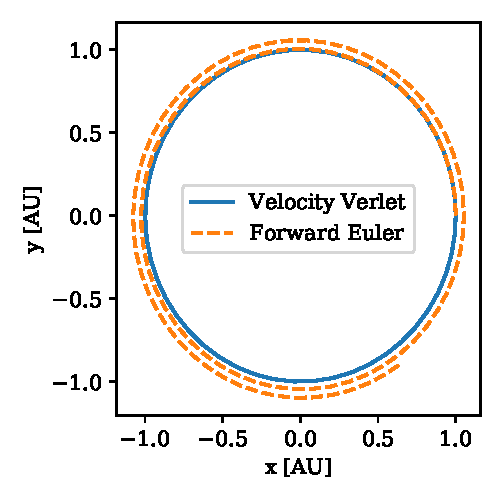
\includegraphics[scale=1]{Figures/circularcomparison.pdf}
\caption{Figure showing the trajectory for the Sun and Earth system initialized with the earth at a distance of $1$AU from the Sun with an initial circular velocity of $6.28$AU/Yr using both the Forward Euler and Velocity-Verlet integration methods. The simulation was run for two years with a timestep of $1500$ steps per year.}
\label{fig:traj}
\end{figure}

\begin{figure*}
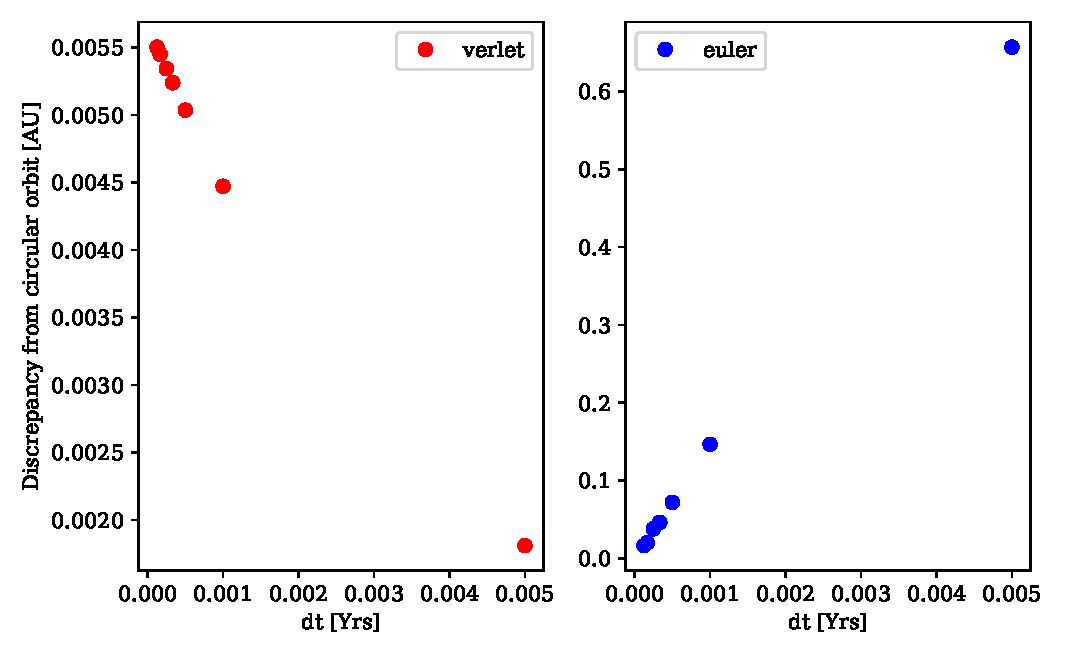
\includegraphics[scale=1]{Figures/taskb_errors.pdf}
\caption{Figure showing the discrepancy between initial starting position in a circular orbit for the Earth in the Sun-Earth system after one orbit as a function of timestep for the Forward Euler method and the Velocity-Verlet method.}
\label{fig:error}
\end{figure*}

\begin{figure}
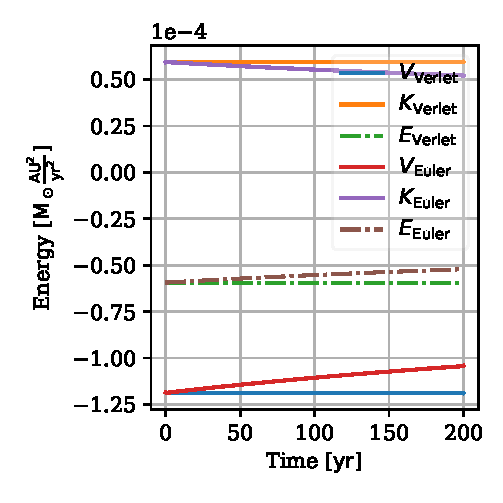
\includegraphics[scale=1]{Figures/taskb_energies.pdf}
\caption{Figue showing the potential and kinetic energy as well as the total energy for the Earth in circular orbit using the Forward Euler and the Velocity Verlet method. The simulation was run over $200$ years using a timestep of $10^5$ steps per year.}
\label{fig:energy}
\end{figure}

\begin{figure}
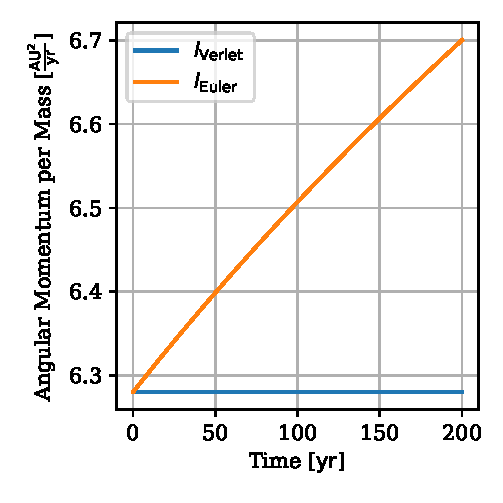
\includegraphics[scale=1]{Figures/taskb_angmom.pdf}
\caption{Figure showing the angular momentum of the Earth in circular orbit sing the Forward Euler and the Velocity Verlet method. The simulation was run over $200$ years using a timestep of $10^5$ steps per year.}
\label{fig:angmom}
\end{figure}

When calculating the escape velocity for the Earth with respect to the Sun, we
found using \ref{eq:v_esc} that the escape velocity for the earth at a distance
of $1$AU to be $8.88$ AU/Yr. The escape velocity was also approximated
numerically. This is shown in Figure \ref{fig:escape}. This result was simulated
using the the Velocity-Verlet method with an initial distance of $1$AU from the
Sun along the $x-$axis with a varying intial velocity in the $y-$direction. The
simulations was run for $1000$ years with a timestep of $1000$ steps per year.
The simulation time of $1000$ years was chosen to make sure the Earth really
escapes and does not get pulled back into orbit after a few years. The
Velocity-Verlet method was also tested with a varying $\beta$ for the exponent
in the radial term of the gravitational law as described in section
\ref{sec:modgrav}. This result is shown in Figure \ref{fig:beta}. Here we
initialized the Earth with a distance of $1$AU from the Sun with a velocity
slightly higher than circular velocity, namely $6.7$AU/Yr. The system was
simulated for one year using $10^4$ timesteps per year.


\begin{figure}
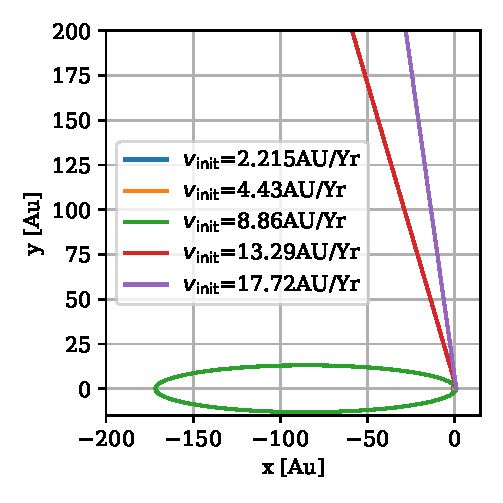
\includegraphics[scale=1]{Figures/espace.pdf}
\caption{Figure showing the trajectory of the Earth in the Earth-Sun system with a varying initial velocity to see wether it reaches escape velocity. The earth is initialized with a distance of $1$AU of the Sun. The simulation was run using the Velocity-Verlet scheme for $1000$ years with a timestep of $1000$ steps per year.}
\label{fig:escape}
\end{figure}

\begin{figure}
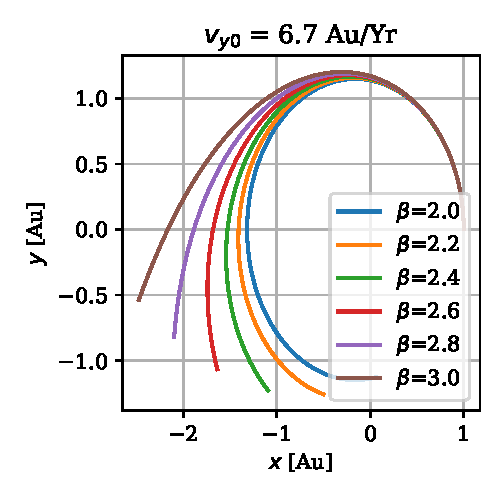
\includegraphics[scale=1]{Figures/beta.pdf}
\caption{Figure showing the trajectory of the Earth in the Earth-Sun system for different $\beta$ as described in section \ref{sec:modgrav}. Here the Earth is initialized at a distance of $1$AU with an initial velocity of $6.7$AU/Yr. Slightly higher than circular orbit. The simulation was run using the Velocity-Verlet scheme for one year using a timestep of $10000$ timesteps per year.}
\label{fig:beta}
\end{figure}


The method was also tested using the Velocity-Verlet scheme for a three body system including the Sun, Earth and
Jupiter. These simulations were initialized using the initial data for the three
objects given by the Horizon-Web interface provided by NASA. The simulations
were run for $15$ years with a timestep of $10000$ steps per year. We also
studied the effect of changing the mass of Jupiter by a factor of $10$ and
$1000$. These results are shown in figures \ref{fig:jupiter},
\ref{fig:jupiter10} and \ref{fig:jupiter1000} respectively. The method was also
expanded to include all the major planets in the Solar system including Pluto as
well as the Tesla Roadster launched by SpaceX. This system was simulated for
$250$ yeas with a timestep of $10000$ steps per year. Figure \ref{fig:outer}
shows the full system while Figure \ref{fig:inner} shows the inner Solar system
as the orbits of the inner planets are barely visible when including the orbits
of the outer bodies. For the inner solar system the simulation was run for three
years with a timestep of $10000$ steps per year.

\begin{figure}
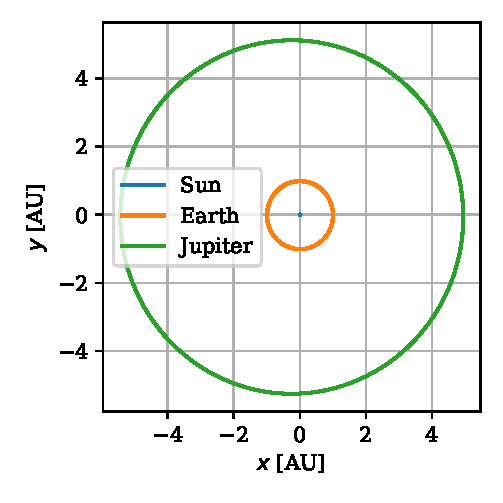
\includegraphics[scale=1]{Figures/jupiter.pdf}
\caption{Figure showing the three-body solution of the Sun, Earth and Jupiter system
with Jupiter having its normal mass. The simulation were initialized using the
initial data for the three objects given by the Horizon-Web interface provided by NASA. The simulations
were run for $15$ years with a timestep of $10000$ steps per year.}
\label{fig:jupiter}
\end{figure}

\begin{figure}
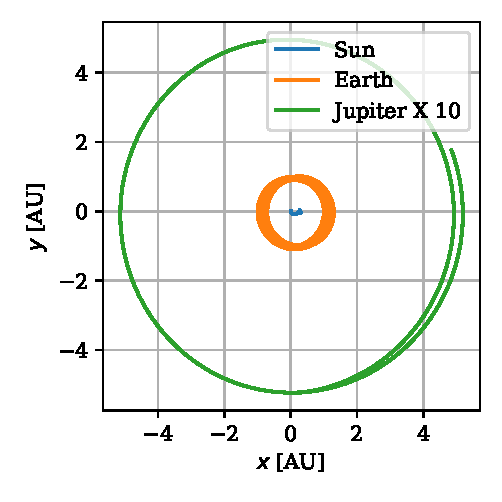
\includegraphics[scale=1]{Figures/jupiter10.pdf}
\caption{igure showing the three-body solution of the Sun, Earth and Jupiter system
with Jupiter having ten times its normal mass. The simulation were initialized using the
initial data for the three objects given by the Horizon-Web interface provided by NASA. The simulations
were run for $15$ years with a timestep of $10000$ steps per year.}
\label{fig:jupiter10}
\end{figure}

\begin{figure}
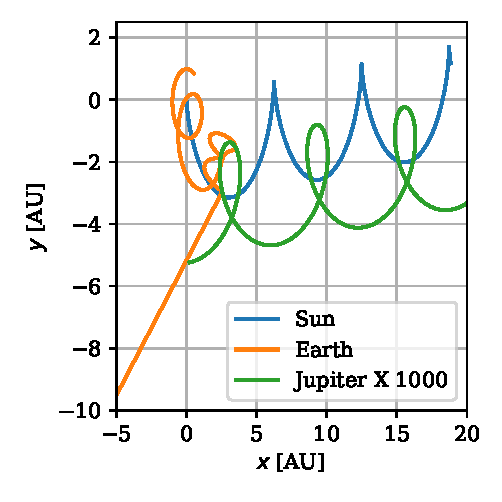
\includegraphics[scale=1]{Figures/jupiter1000.pdf}
\caption{igure showing the three-body solution of the Sun, Earth and Jupiter system
with Jupiter having $1000$ times its normal mass. The simulation were initialized using the
initial data for the three objects given by the Horizon-Web interface provided by NASA. The simulations
were run for $15$ years with a timestep of $10000$ steps per year.}
\label{fig:jupiter1000}
\end{figure}

\begin{figure*}
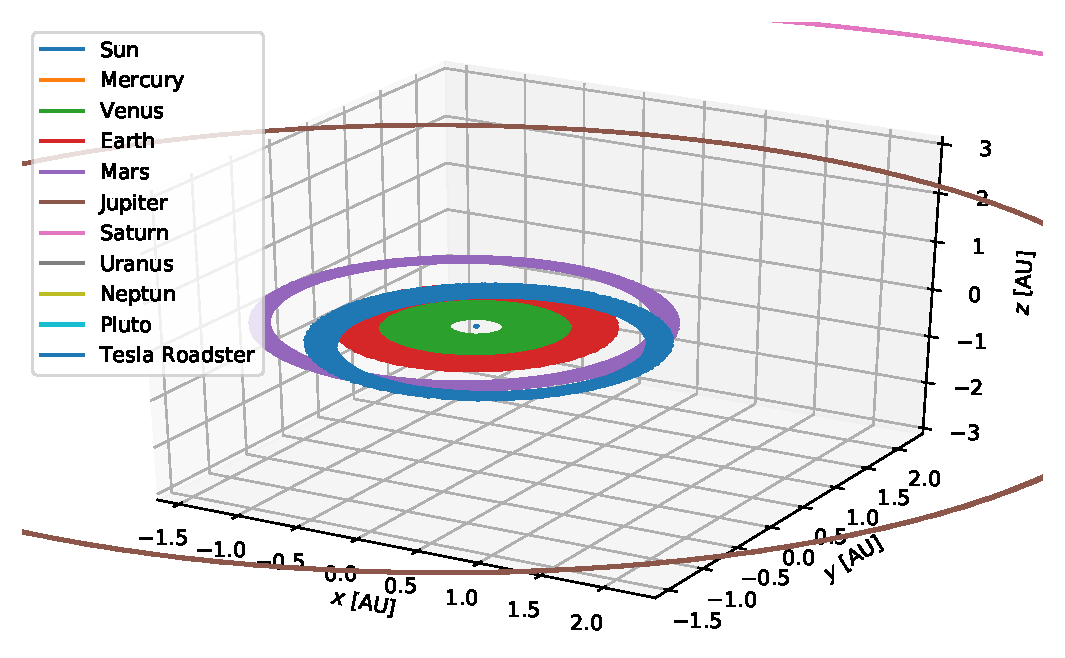
\includegraphics[scale=1]{Figures/InnerSolarSystem.pdf}
\caption{Figure Showing a solution for the inner Solar system using the Velocity-Verlet scheme. The simulation was run for three years with a timestep $10000$ steps per year. The initial data was given by the Horizon-Web interface provided by NASA}
\label{fig:outer}
\end{figure*}

\begin{figure*}
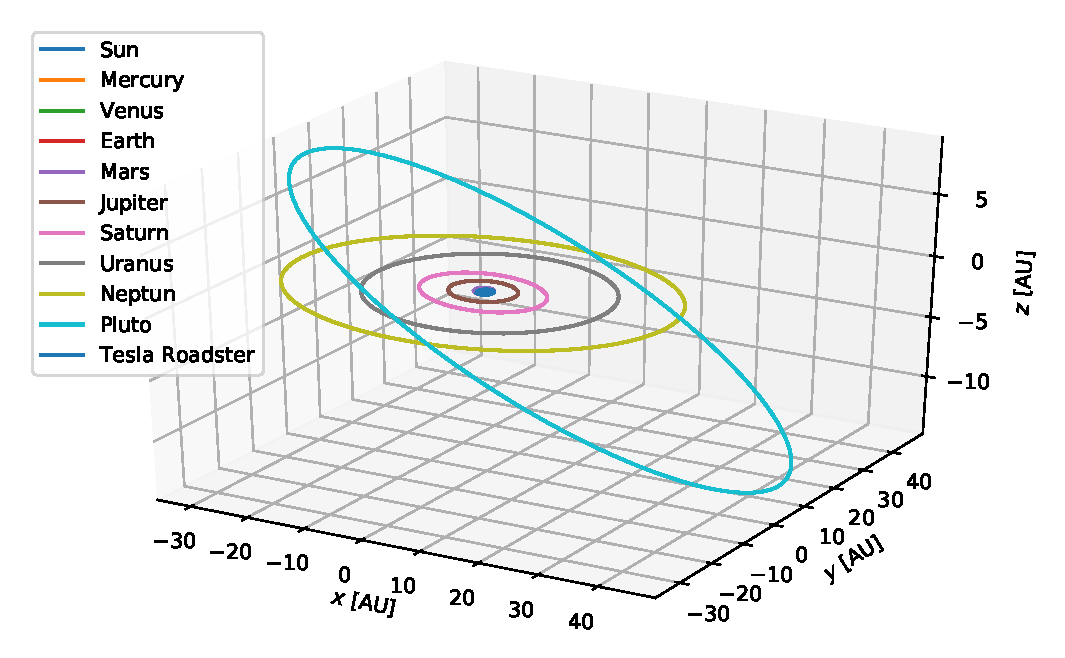
\includegraphics[scale=1]{Figures/OuterSolarSystem.pdf}
\caption{Figure Showing a solution for the full Solar system using the Velocity-Verlet scheme. The simulation was run for $250$ years with a timestep $10000$ steps per year. The initial data was given by the Horizon-Web interface provided by NASA}
\label{fig:inner}
\end{figure*}

The perihelion precession of Mercury was also calculated using the general
relativistic correction term to the newtonian force given by
\ref{eq:relcorrection} as discussed in section \ref{sec:mercuryprecession}. The
precession per century was found to be approximately $450399$ arcseconds with
the relativistic correction term and $450420$ withouth the correction term. This
result was calculated over $100$ years with a step size of $10^7$ steps per year.

\section{Discussion} \label{sec:discussion}
As seen in the orbits in Figure \ref{fig:traj}, the Verlet method 
keeps the Earth in a circular orbit, while the Euler method seems to 
increase the total energy of the system as its orbital radius increases 
with time. This is expected behaviour, as Verlet is known to be better
at conserving energy than Euler. This observation also consistent with 
Figure \ref{fig:energy}. This figure shows that 
Euler increases the total energy over time, decreasing the kinetic energy
and increasing the potential energy as the Earth moves away from the Sun. 
We also see in Figure \ref{fig:angmom} that Euler does not conserve angular 
momentum over time compared to Verlet.
An interesting detail in the discrepancies shown in Figure \ref{fig:error}
is that the error increases with smaller time-steps within the range 
shown. This makes sense as errors in numerical schemes can be decomposed 
into \begin{equation}
\mathrm{err}_\mathrm{tot}=\mathrm{err}_\mathrm{Taylor} + \mathrm{err}_
\mathrm{Numerical}, \label{eq:error_decomp}
\end{equation} where $\mathrm{err}_\mathrm{Taylor}$ is the error from the 
Taylor series used to derive the numerical scheme and $\mathrm{err}_
\mathrm{Numerical}$ is the error caused by numerical round off. A 
possible explanation for this is that
$\mathrm{err}_\mathrm{Taylor} \ll \mathrm{err}_\mathrm{Numerical}$, 
and the numerical round off error increases with decreasing time step. 
The total error is clearly better for the Velocity Verlet scheme in 
this case, the error for Euler being several orders of magnitude 
higher. In addition the Velocity Verlet and Euler schemes seem to have 
very similar run times, meaning there is no argument for not using 
Verlet instead of Euler in this case.

When researching gravitational forces with different radial power laws, 
the results shown Figure \ref{fig:beta} seem to be consistent with 
Bertrand's theorem as discussed in Section \ref{sec:modgrav}, 
showing that only the Sun-Earth-system with gravity $F_g\propto R^{-2}$ 
has a closed orbit. According to the theorem all the shown systems will 
be bound, but only the Newtonian gravitational force with $\beta=2$ will 
have a closed orbit. For $\beta>2$ we expect a perihelion precession. 
The Earth's orbit for $\beta>2$ will experience a  
weaker gravitational force and will drift further out before returning 
towards the sun. It will not return to same initial starting point, but 
will instead have a precession motion around the Sun if it doesn't 
escape. One could however expect that at a smaller distance, let's 
say if we were to simulate a Sun-Mercury-system, the force could increase 
for $\beta>2$ as $R<1$ AU.

Figure \ref{fig:escape} shows that the escape velocity is somewhere 
in the range $v\in(8.86, 9.5)$ AU/Yr, which corresponds well with 
the analytical escape velocity $v\approx 8.88$ AU/Yr. Whether this theoretical 
velocity is the escape velocity in this simulated system is unclear 
though, as it may not be accurate enough to recreate this.

When simulating the Sun-Earth-Jupiter-system with regular masses and 
initial values from \cite{nasa:2019} as shown in Figure 
\ref{fig:jupiter} we see that system behaves as observed in nature 
where all three bodies exhibit closed, stable orbits around the CM.
Increasing the mass of Jupiter in the Sun-Earth-Jupiter-system makes the 
system behave increasingly chaotically, especially at 
$1000 \cdot M_\mathrm{\jupiter}$. At ten times the normal mass, 
Jupiter visibly affects the orbit of the Earth. This is easily spotted  
when comparing Figure \ref{fig:jupiter} and \ref{fig:jupiter10}. Every 
time the Earth aligns with Jupiter it will receive a larger gravitational tug than if Jupiter has its regular mass. This system may settle in a new equilibrium in the future, but our results is not sufficient enough to determine whether this will happen. It is also worth noting that our initial data is gathered from a stable system where Jupiter has its regular mass. Therefore it is expected that the system initially behaves unstable as it not in an equilibrium state. Note also that the Sun, usually orbiting a common CM, now ends up in a larger distance from the new CM in its orbital motion. 
In Figure \ref{fig:jupiter1000} Jupiter has a mass very similar to $M_\odot$, meaning the system devolves 
into a chaotic three body system. One can see that the Sun and Jupiter settles into a stable system where both orbit a common CM. The earth however is put into a very unstable orbit experiencing gravitational force from two bodies approximately $10^6$ times as massive. The initial starting point for the Earth would be an equilibrium if Jupiter has its regular mass. Instead with Jupiter having $1000$ times its original mass, we have effectively added another Sun into the system. This will massively perturb the motion of Earth and it will sooner or later experience a close encounter with one of the other bodies being ejected from the system. This may also have resulted in a collision. Our method  has not implemented any collisional effects and since we treat our bodies as point masses a real collision would result in a small radial distance resulting in a large force amplifying the slingshot effect.

The simulation of all planets in the solar system in addition to Pluto and 
the Tesla Roadster launched by SpaceX, as seen in figures \ref{fig:outer} and \ref{fig:inner}, stays visibly stable for several years. Pluto seems to 
have a closed orbit, and keeps its inclination. This indicates that 
the Velocity Verlet scheme is well enough suited for visualisations of this scale. 
If the simulations shown in Figure \ref{fig:outer} and \ref{fig:inner} 
were run using Euler, We have seen from Figure \ref{fig:traj} that the orbits would spiral outwards due to Forward Euler adding to the total energy. In order to have Pluto complete one full orbit we had to simulate for $250$ years. During this time the inner planets of the Solar system would have completed many orbits and would have been perturbed by the spiralling motion. This could result in possible close encounters with either themselves or the outermost massive planets destabilizing the system. However the fact that the inner solar system stays stable for $250$ years is a strong indication that the Velocity Verlet scheme remains stable. The added low-mass Tesla Roadster behavies very similar to the other planets in its orbital motion. However, in a possible future fly-by, it could gain enough angular momentum from one of the planets to achieve escape velocity.

As mentioned when discussing the results in Figure \ref{fig:beta}, a 
inverse-power $\beta>2$ will lead to a perihelion precession. This is effectively 
what happens when adding the relativistic correction term as shown in 
(\ref{eq:relcorrection}), as the correction term has $\beta=4$. This 
will slightly perturb the closed elliptical orbit.
We expected the precession of the Sun-Mercury system to be $\sim 43''$, 
but our results vary dramatically from this. This could imply that our 
simulations aren't accurate enough to resolve details down to this small 
scale. However, as we have simulated Mercury's orbit with a time step of 
$10^{-7}$ years, we should observe an accurate estimate of the perihelion 
precession. This is not the case, indicating that there are systematic 
errors in our integrator or in the post-processing of the data. Perhaps 
there is also some undetected systematic error in the implementation of 
our method. This is something that is important to look 
more into in the future. Other potential sources of the observed 
discrepancy could be a perihelion precession inherent to the Velocity 
Verlet scheme. In order to resolve the motion in a high enough detail the 
timestep had to be low enough in order to measure any significant small 
scale motions like the precession of mercury. We can also see from Figure 
\ref{fig:error} that in our implementation of the velocity-verlet scheme, 
this will also increase the error in the orbital motion resulting in 
motions that may drown the precession motion we were supposed to measure.




\section{Conclusion} \label{sec:conclusion}
We have created an $N$-body simulator implementing Newton's law of 
gravitation and tested it on a solar system scale. Our results imply 
that our method performs well on these larger scales, but struggles to 
resolve small scale motions needed to estimate the perihelion precession 
of Mercury.

In the future collision modelling should be added to better simulate 
chaotic systems such as a three body problem with equally large masses. 
Time should be invested in exploring possible reasons for the systematic 
errors causing us to not properly estimate the perihelion precession 
of Mercury. Also, the timing comparing the Euler and Velocity Verlet 
schemes should be done many times and then averaged to get a better 
estimation of their performance relative to each other.
\nocite{jensen:2019}
\newpage
\bibliography{ref}
\bibliographystyle{aasjournal}
\end{document}

% End of file `sample62.tex'.
